\documentclass[11pt, english]{article}

\usepackage[
top    = 2.5cm,
bottom = 2.5cm,
left   = 2.5cm,
right  = 2.5cm]{geometry}

%\documentclass[oneside,a4paper,10pt,english, english]{book}
\usepackage[latin1]{inputenc}
\setlength\parskip{\medskipamount} \setlength\parindent{0pt}
\usepackage{amsmath}
\usepackage{setspace}
\usepackage{babel}
\usepackage{amssymb}
\usepackage{float}
\usepackage{graphicx}
\usepackage{filecontents}
\usepackage{subcaption}
\usepackage[export]{adjustbox}
\usepackage{booktabs}
\errorcontextlines 10000
\pretolerance=10000
\newcommand{\lsim}{\raisebox{-1.5mm}{$\:\stackrel{\textstyle{<}}{\textstyle{\sim}}\:$}}

\begin{document}

In addition to using traditional cuts (Higgs combined tool) to set upper limits on Z'2HDM and Z'Baryonic models, a multivariate analysis using discriminants from a Bayesian Neural Network (BNN) was used. For an overview and example of how a Bayesian framework fits with a neural network, see Bayesian Neural Networks \cite{BNN:1}. To capture the best results, three different Bayesian discriminants were created, each using unique variables in their discriminants. The performance of two of these discriminants is is Figure \ref{fig: Dperform}.

\begin{figure}[h!]
	\begin{subfigure}{.5\textwidth}
		\centering
		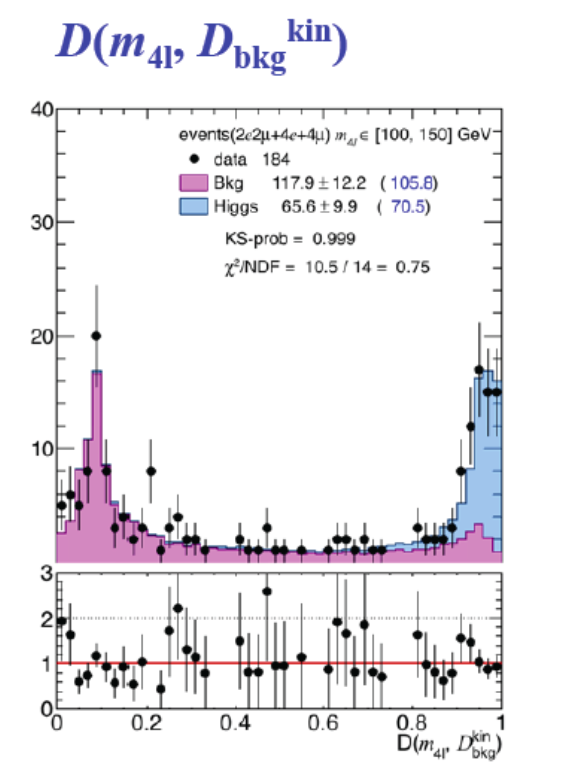
\includegraphics[width = .7\linewidth, height = 12 cm, keepaspectratio]{/Users/alexstoken/projects/monoHiggs/latexHiggs/Dtwo.png}
		\caption{$D(m_{4\ell}, D_{kin}^{bkg})$}
		\label{fig: D2}
	\end{subfigure}%
	\begin{subfigure}{.5\textwidth}
		\centering
		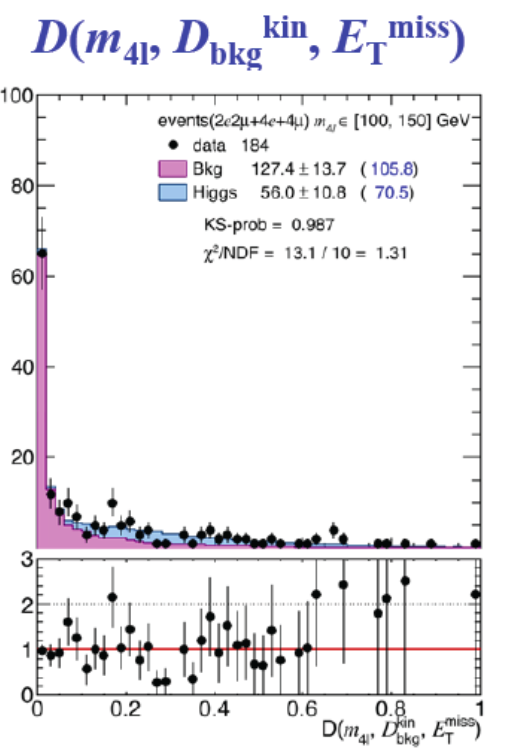
\includegraphics[width = .61\linewidth, height = 11 cm, keepaspectratio]{/Users/alexstoken/projects/monoHiggs/latexHiggs/Dthree.png}
		\caption{$D(m_{4\ell}, D_{kin}^{bkg}, E_{T}^{miss})$}
		\label{fig: D3}
	\end{subfigure}
	
	\caption{Performance of Discriminants}
	\label{fig: Dperform}	
\end{figure}

\begin{figure}[b!]
	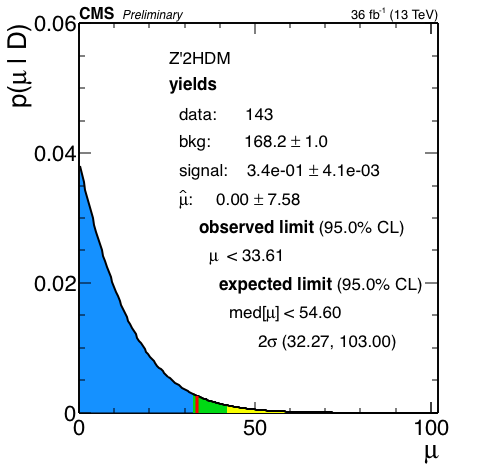
\includegraphics[height = 7 cm, keepaspectratio, center]{/Users/alexstoken/projects/monoHiggs/latexHiggs/indivLimit.png}
	\caption{Upper limit on Z'2HDM with $m_{Z'} = 600 GeV, m_{A0} = 300 GeV $}
	\label{fig: indvlimit1}
\end{figure}


From this preliminary result, it appears that the $D(m_{4\ell}, D_{kin}^{bkg})$ can better differentiate between Higgs events and background events. Nevertheless, both were used to set upper limits.

To produce the limits for each model, a Bayesian approach was again used, this time on $\mu$. Bayesian statistics rely on given prior probabilities to predict the probability of data fitting a model and, in turn, of a model fitting data. To keep this analysis as general as possible and avoid any unintended bias, a flat prior was used. This Bayesian analysis was done on each individual model (with varied masses of Z' and it's decay products) for a 95\% confidence interval. An example of an individual limit on $\mu$ is shown in Figure \ref{fig: indvlimit1}.

Combining the observed $\mu$ with the branching ratio and cross sections for each model has yielded upper limits, with 95\% confidence, on Z'2HDM and Z'baryonic models. In addition to the three BNN discriminants  $D(E_{T}^{miss}), D(m_{4\ell}, D_{kin}^{bkg}), D(m_{4\ell}, D_{kin}^{bkg},  E_{T}^{miss})$ used to set upper limits, $E_{T}^{miss}$ and $P_{T4\ell}$ were also used in the Bayesian analysis to set limits. The upper limits differed depending on which variable was used to set them, and these differences can be seen in  Table \ref{table: lims_difmethods} for Z'Baryonic $m_{Z'}= 95$ , $m_{\chi} = 50$. Note that these are the limits before being weighted by their specific branching ratio and cross section. Smaller limits are better. 

\begin{table}[h]
	\centering
	\begin{tabular}{cccccc}
	\toprule
	Value & $E_{T}^{miss}$ & $P_{T4\ell}$ & $D(E_{T}^{miss})$ & $D(m_{4\ell}, D_{kin}^{bkg})$ & $D(m_{4\ell}, D_{kin}^{bkg}, E_{T}^{miss})$\tabularnewline
	\midrule
	Observed & 18.231 & 25.764 & 41.898 & 104.778 & 37.358\tabularnewline
	$-2\sigma$ & 18.713 & 26.003 & 42.280 & 103.086 & 37.913\tabularnewline
	$-\sigma$ & 20.624 & 28.943 & 52.733 & 134.193 & 47.448\tabularnewline
	Expected & 26.121 & 33.710 & 70.289 & 172.855 & 63.037\tabularnewline
	$+\sigma$ & 33.386 & 42.715 & 102.172 & 257.193 & 84.345\tabularnewline
	$+2\sigma$ & 42.389 & 51.528 & 136.672 & 324.874 & 115.923\tabularnewline
	\bottomrule
	\end{tabular}
	\caption{$\mu$ values for Z'Baryonic $m_{Z'}= 95$ , $m_{\chi} = 50$}, 
	\label{table: lims_difmethods}
\end{table}
The table shows us that discriminants without kinematic variables do are not sensible to limit our models. Instead, traditional approaches like $E_{T}^{miss}$ and $P_{T4\ell}$ set the lowest limits, along with a well made discriminant $D(m_{4\ell}, D_{kin}^{bkg}, E_{T}^{miss})$ based off of these variables. At this time, systematic uncertainties associated with these variables are not included in these limits, and that those uncertainties will propagate to the discriminants. The BNN itself, however, does not have any systematic uncertainty associated with it. These limits are easier to visualize graphically. Below in Figure \ref{fig: limitsPlots} are limits on Z' $m_{A0} = 300$ and Z'Baryonic $m_{\chi} = 1$ (the Z'Baryonic model used for the combined channel monoHiggs analysis) made with $E_{T}^{miss}$ as the limiting variable.
\begin{figure}[H]
	\begin{subfigure}{.5\textwidth}
		\centering
		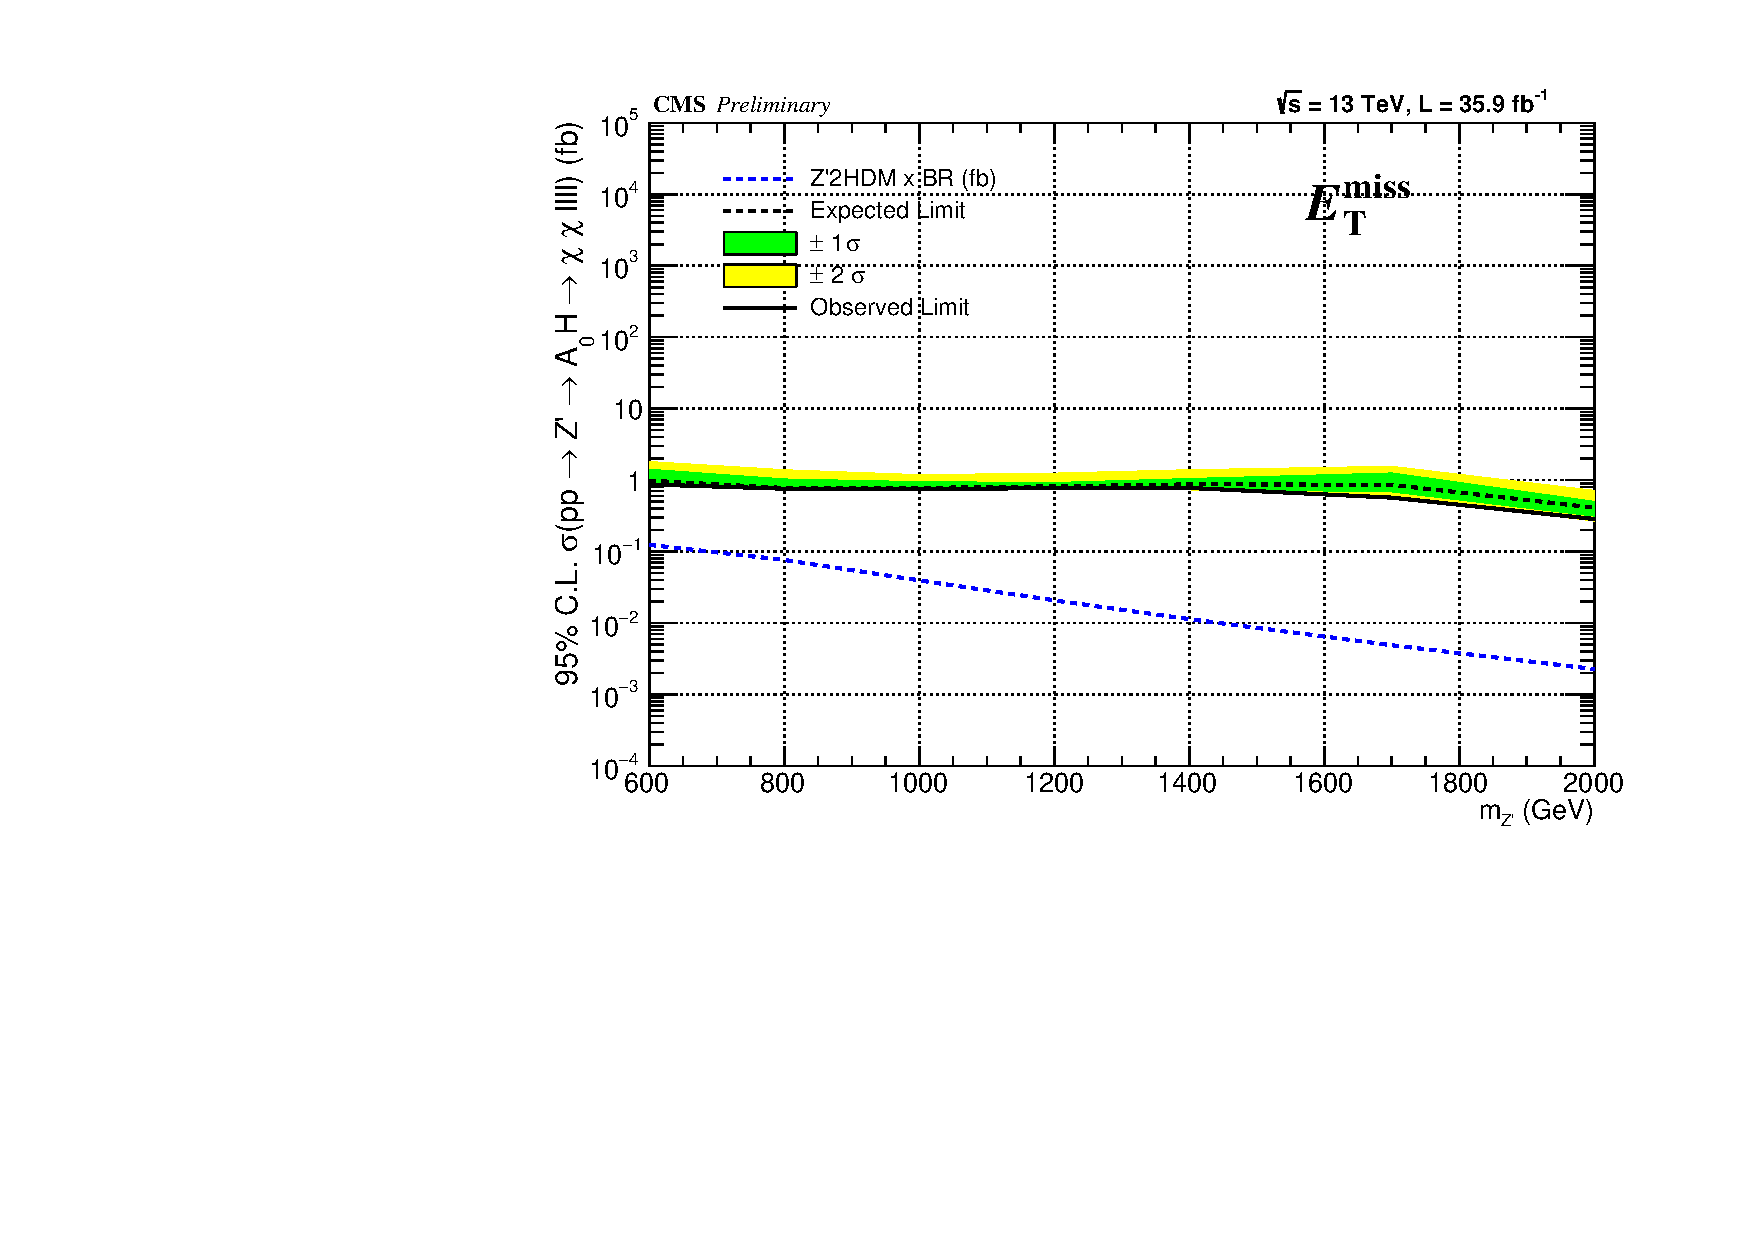
\includegraphics[height = 5.5 cm, keepaspectratio, center]{/Users/alexstoken/projects/monoHiggs/latexHiggs/limZprimeMET300.pdf}
		\centering
		\caption{Z'2HDM $m_{A0} = 300$}
		\label{fig: limZprime300met}
	\end{subfigure}%
	\begin{subfigure}{.5\textwidth}
		\centering
		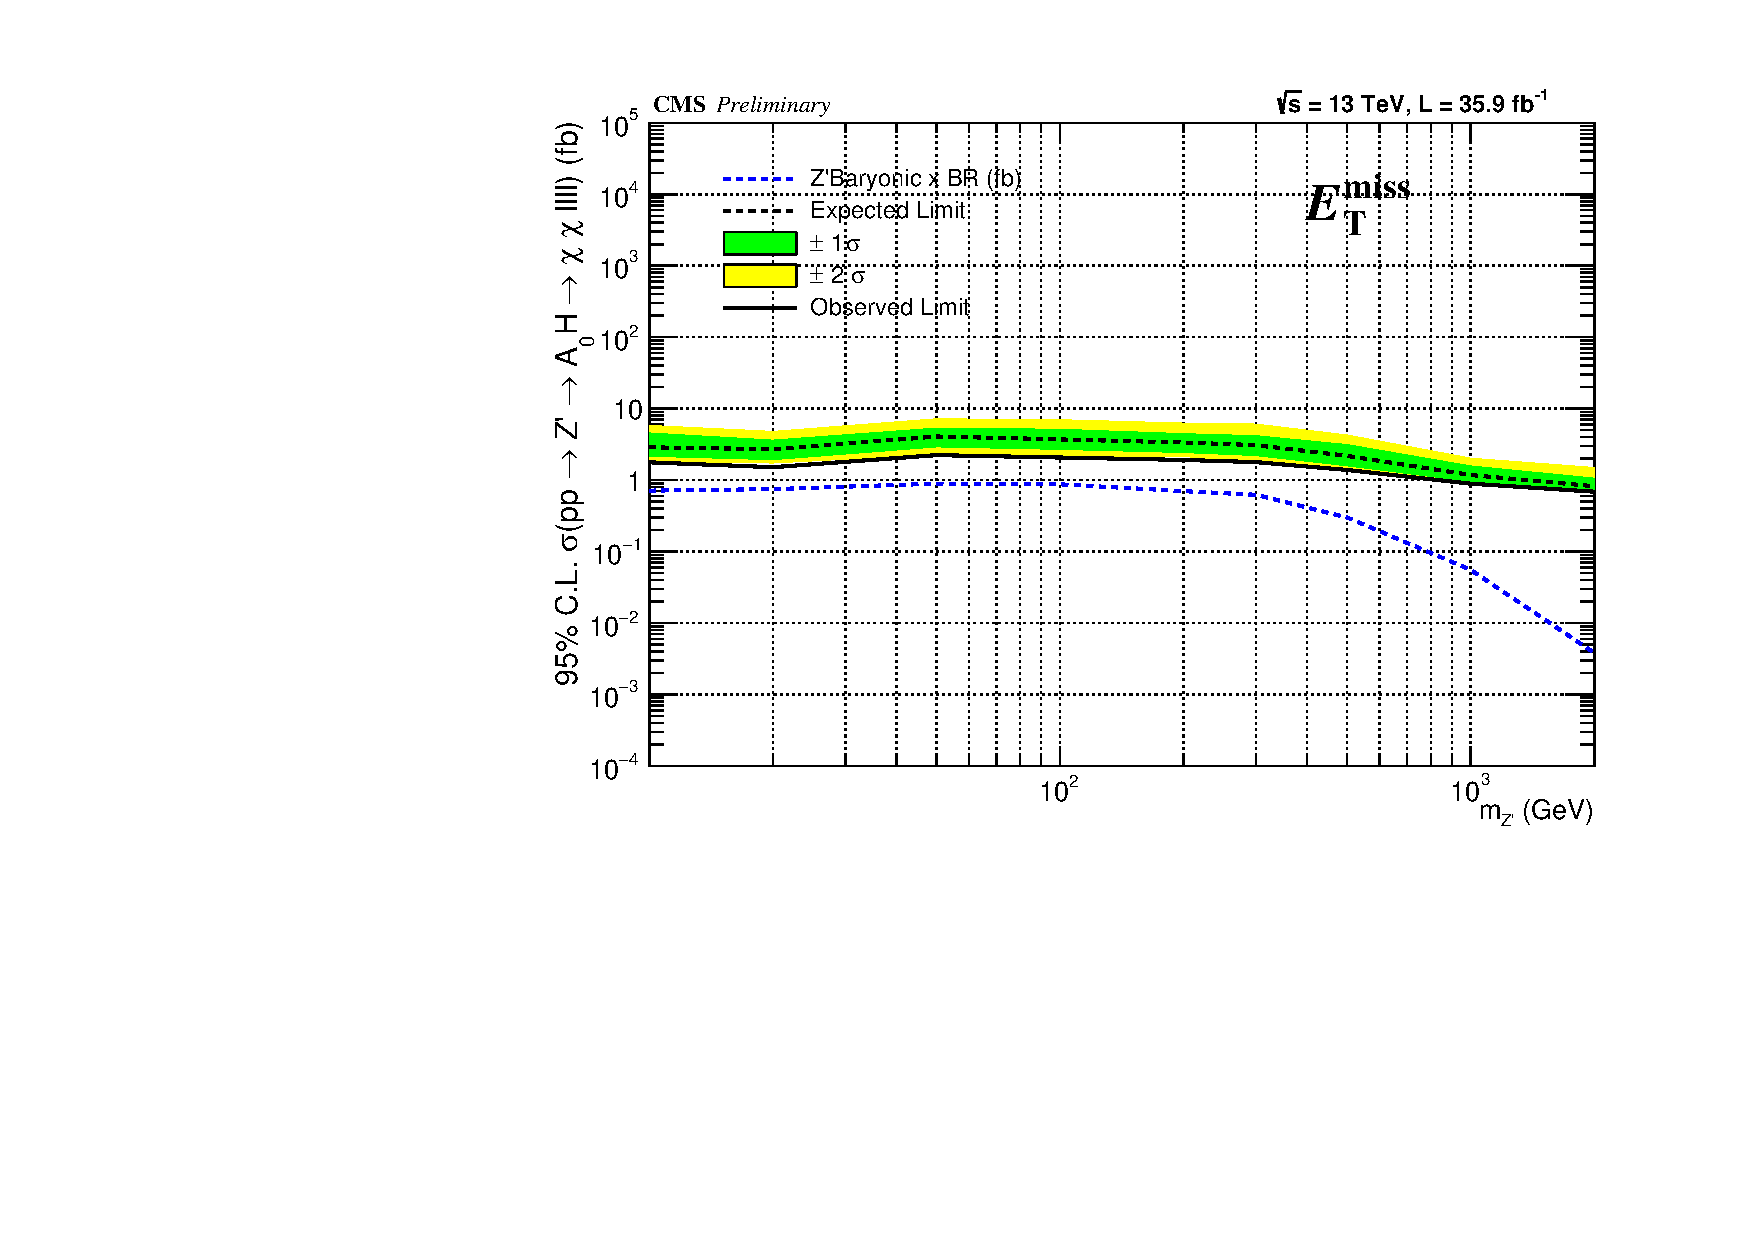
\includegraphics[height = 5.5 cm, keepaspectratio, center]{/Users/alexstoken/projects/monoHiggs/latexHiggs/limZpBaryMET1.pdf}
		\caption{Z'Baryonic $m_{\chi} = 1$}
		\label{fig: limZpBary1met}
	\end{subfigure}
\caption{Upper limits on models using $E_{T}^{miss}$}
\label{fig: limitsPlots}
\end{figure}

Here we can see the limits on various mass models with the given $m_{A0}$ and $m_{\chi}$ produced. The goal of the analysis is to get the limits under 1, since is this the exclusion range (where we can say that a model is so unlikely that it no longer merits consideration). From these plots, it is apparent that the models centered around a higher mass Z' are getting closer to the exclusion range, although they are not there yet. With more events from the HL-LHC, the limits on many of these models will move toward and below the threshold for exclusion. At this time, systematic uncertainties are not considered in the limits, so the limits are being recalculated.

What follows is a graphical comparison of the limits gathered through a Bayesian analysis on several variables. Most notable will be the comparison between limits produced by $E_{T}^{miss}$, $P_{T4\ell}$, and $D(m_{4\ell}, D_{kin}^{bkg}, E_{T}^{miss})$. 

\begin{figure}[h!]
	\begin{subfigure}{.5\textwidth}
		\centering
		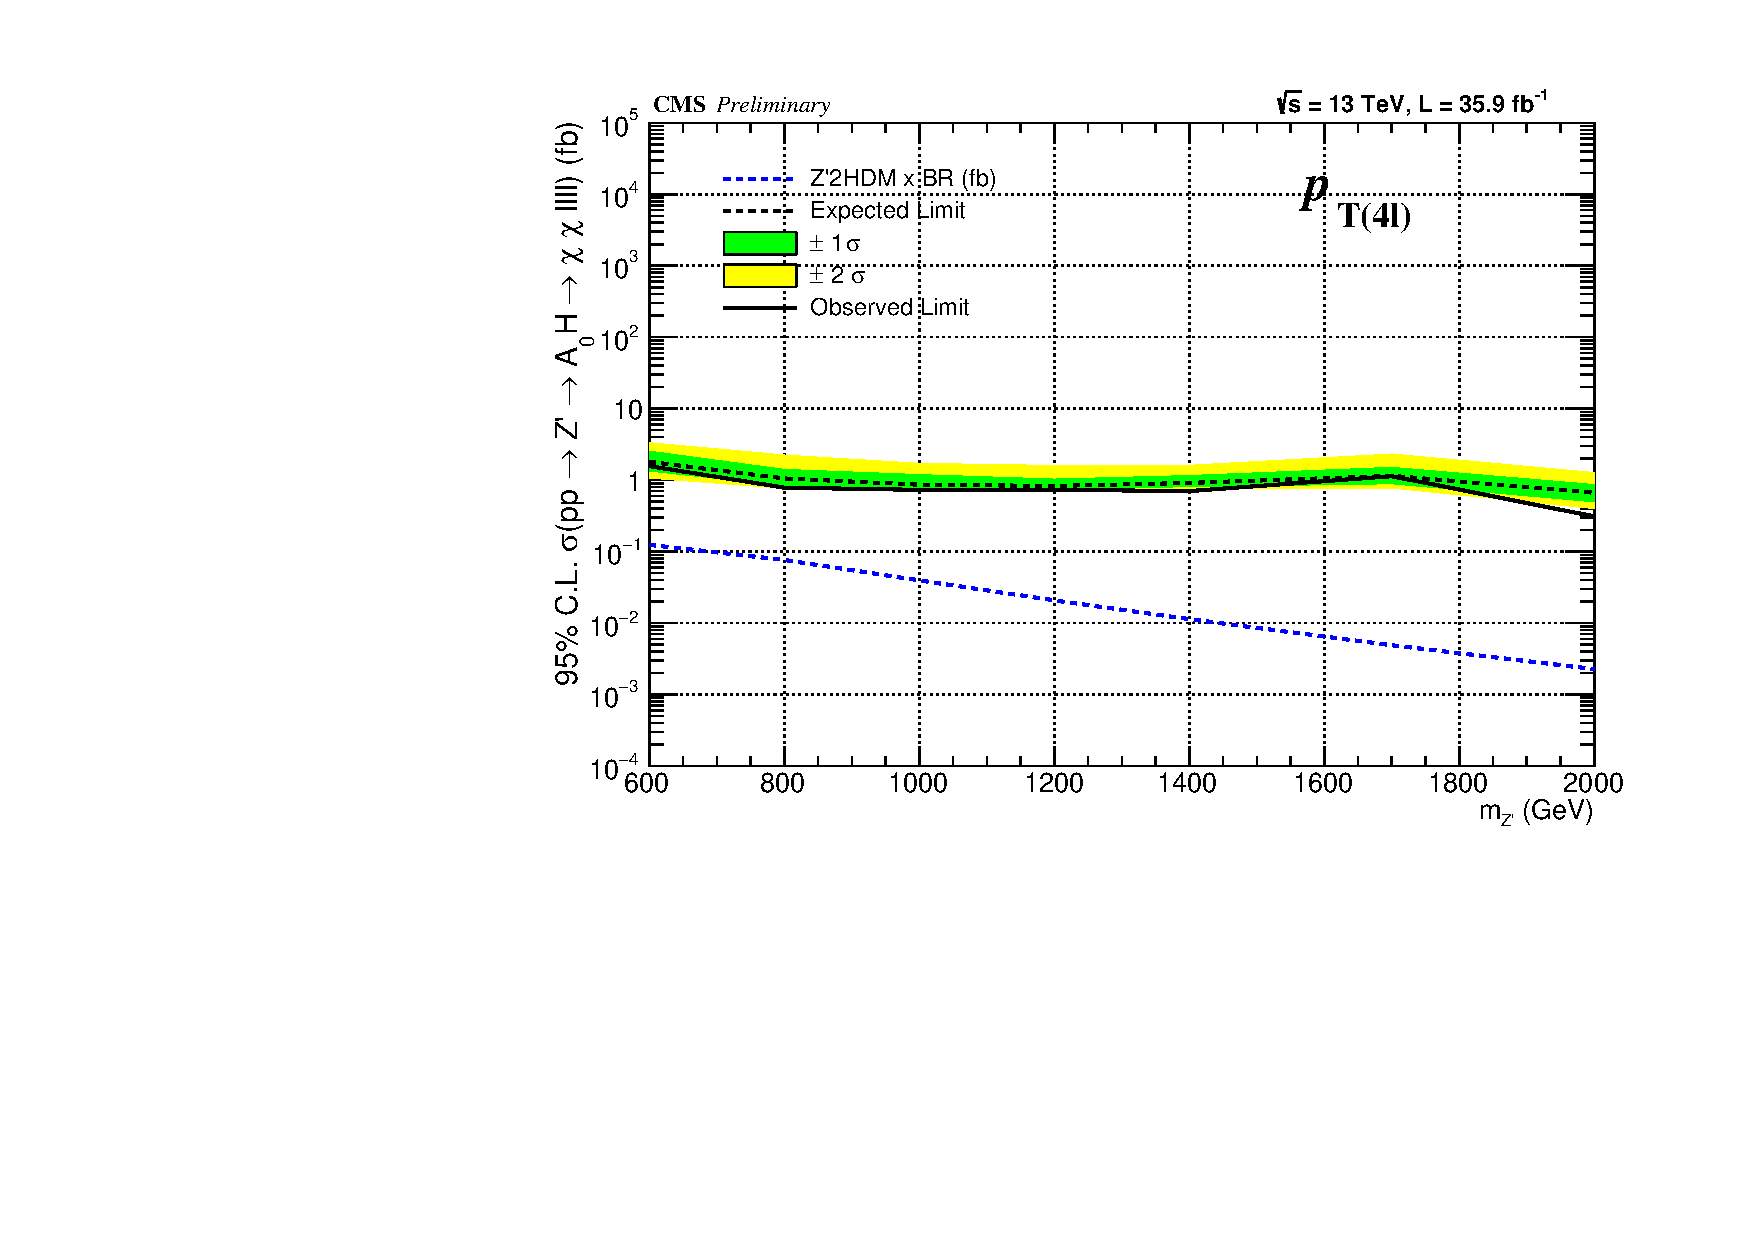
\includegraphics[height = 5.5 cm, keepaspectratio, center]{/Users/alexstoken/projects/monoHiggs/latexHiggs/limZprimePT4L300.pdf}
		\centering
		\caption{Z'2HDM $m_{A0} = 300$}
		\label{fig: limZprime300pt4l}
	\end{subfigure}%
	\begin{subfigure}{.5\textwidth}
		\centering
		\includegraphics[height = 5.5 cm, keepaspectratio, center]{/Users/alexstoken/projects/monoHiggs/latexHiggs/limZpBaryPT4L1.pdf}
		\caption{Z'Baryonic $m_{\chi} = 1$}
		\label{fig: limZpBary1pt4l}
	\end{subfigure}
\caption{Upper limits on models using $P_{T4\ell}$}
\label{fig: limitsPlotsPT4l}
\end{figure}

\begin{figure}[h!]
	\begin{subfigure}{.5\textwidth}
		\centering
		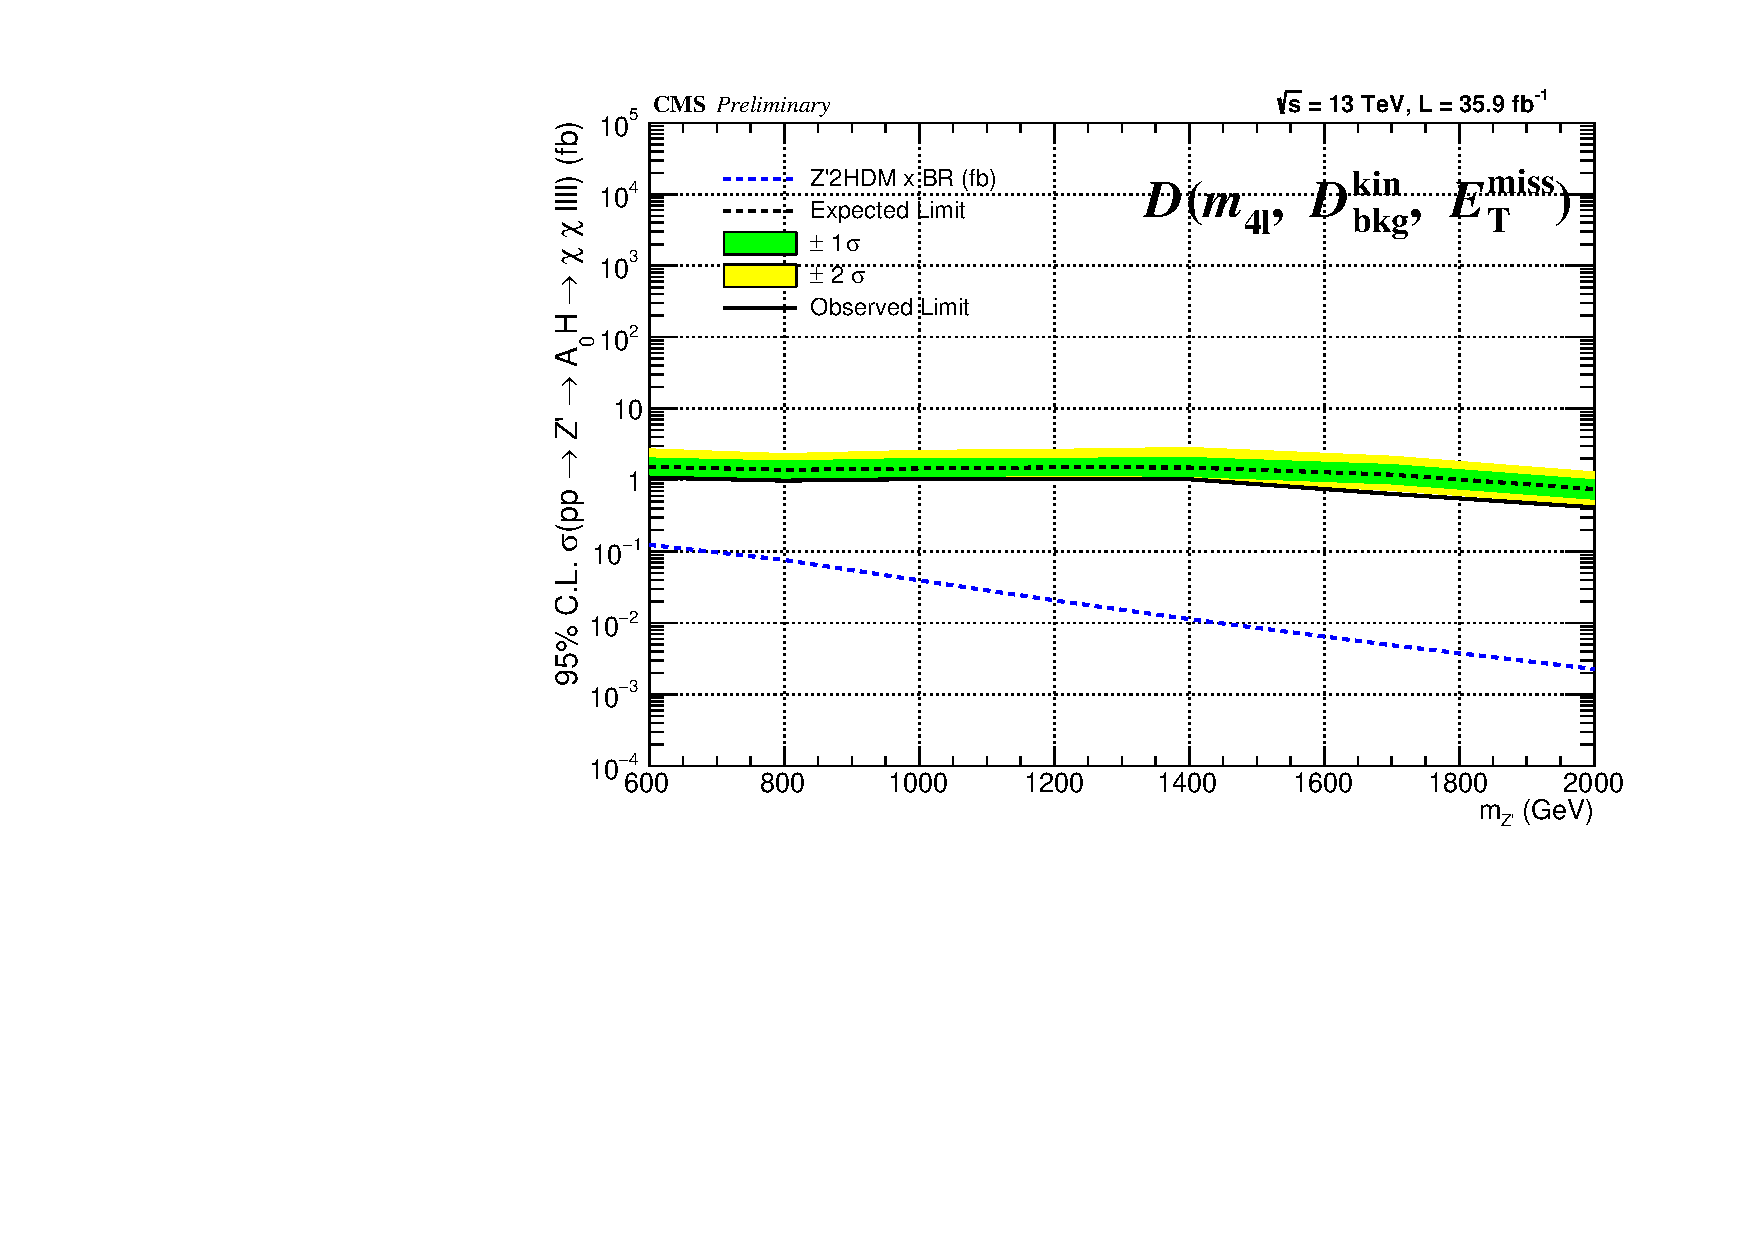
\includegraphics[height = 5.5 cm, keepaspectratio, center]{/Users/alexstoken/projects/monoHiggs/latexHiggs/limZprimeD3300.pdf}
		\centering
		\caption{Z'2HDM $m_{A0} = 300$}
		\label{fig: limZprime300D3}
	\end{subfigure}%
	\begin{subfigure}{.5\textwidth}
		\centering
		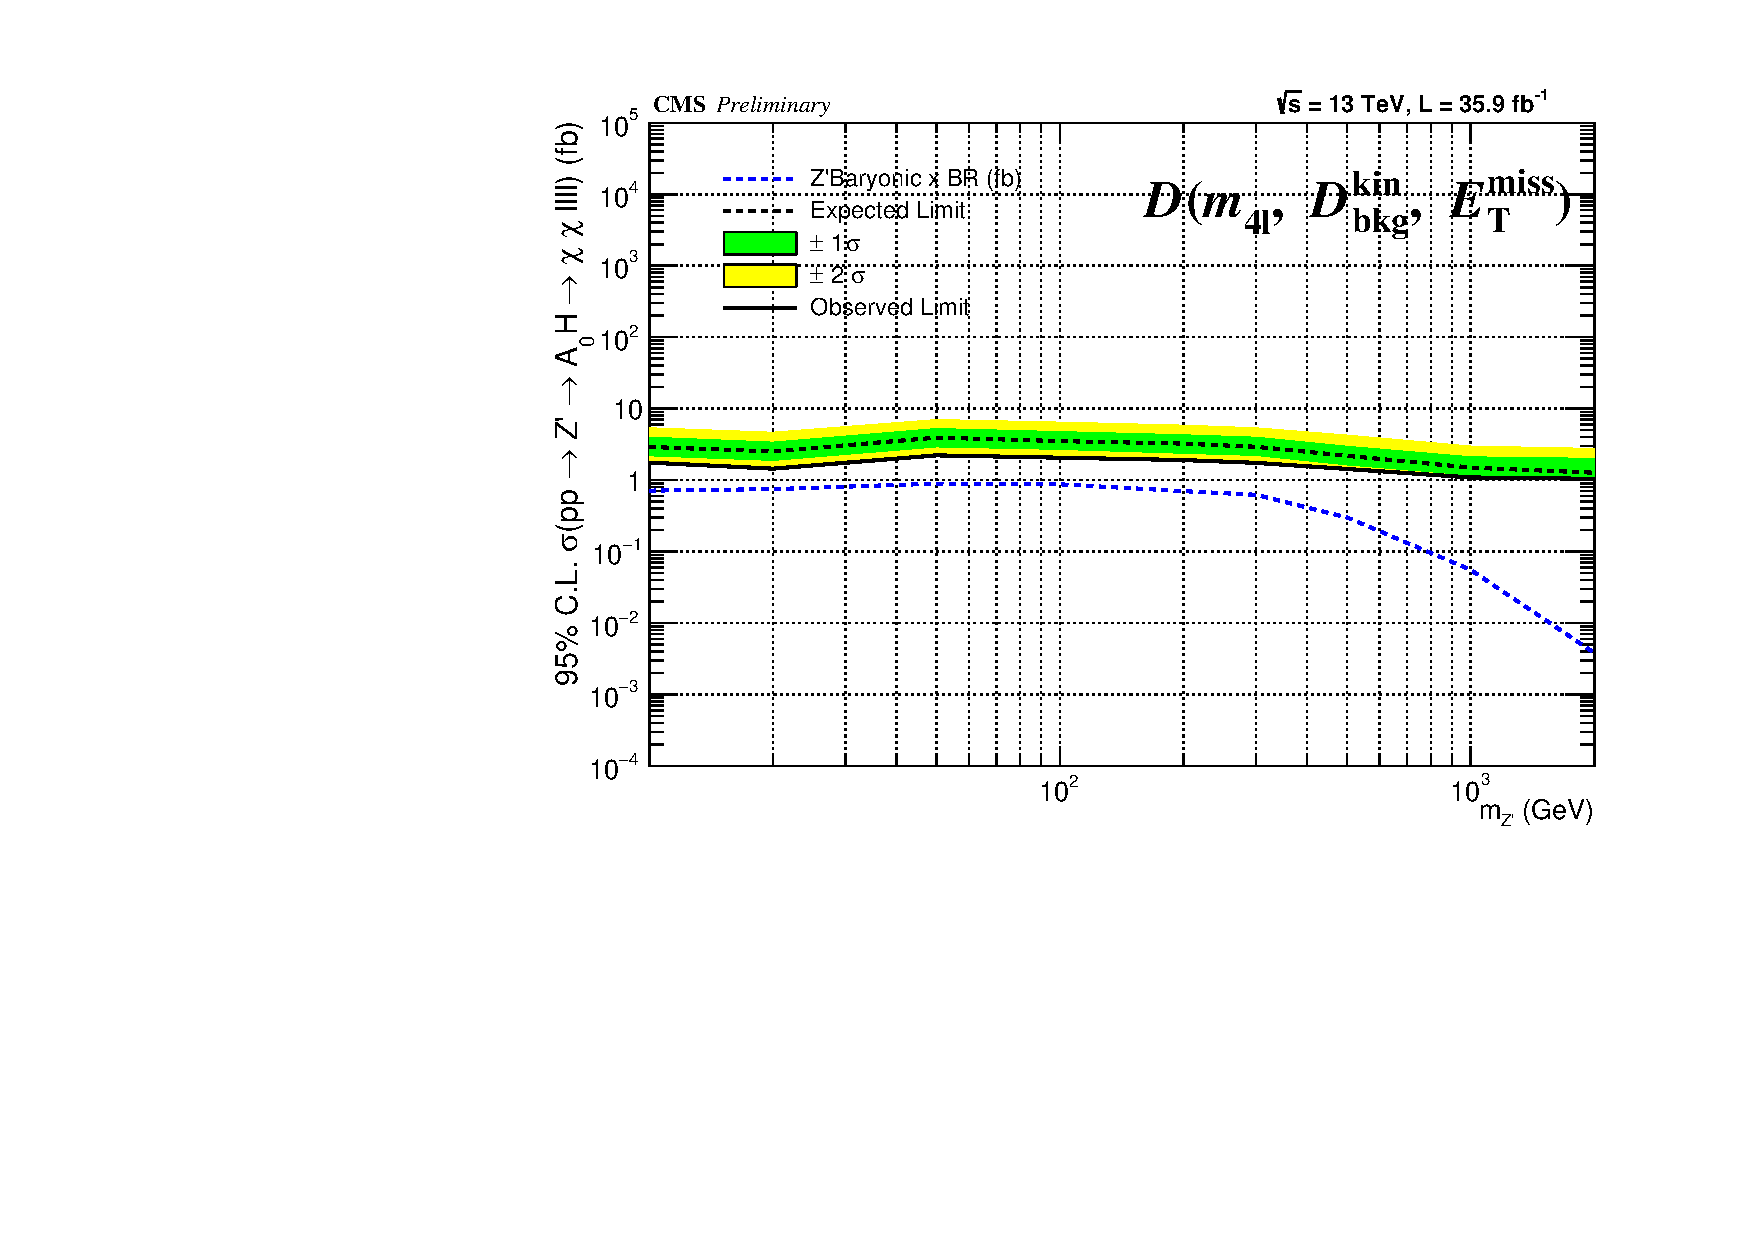
\includegraphics[height = 5.5 cm, keepaspectratio, center]{/Users/alexstoken/projects/monoHiggs/latexHiggs/limZpBaryD31.pdf}
		\caption{Z'Baryonic $m_{\chi} = 1$}
		\label{fig: limZpBary1D3}
	\end{subfigure}
\caption{Upper limits on models using $D(m_{4\ell}, D_{kin}^{bkg}, E_{T}^{miss})$}
\label{fig: limitsPlotsD#}
\end{figure}

A quick analysis of these limits shows that the plots for each model retain the same shape, despite the variable used to form the limits. The discriminant does soften the limit curve when compared to the single kinematic factors, which is to be expected. This comparison does, to some degree, shed light on which variable is the most effective for setting limits. While $E_{T}^{miss}$ is the most commonly accepted kinematic variable, it's high systematic uncertainty leaves room for $P_{T4\ell}$ to be an almost equally, of not more effective, variable in limit setting. The possibility of $P_{T4\ell}$ as a useful limiter is currently an area of current interest and will continue to be explored by creating discriminants with $P_{T4l\ell$ instead of and alongside $E_{T}^{miss}$, and testing their performance. 

\newpage

\bibliography{monoHiggs}
\bibliographystyle{plain}

\end{document}






